\documentclass[12 pts]{article}
\usepackage{graphicx}
\usepackage{wrapfig}
\usepackage{mathtools}
\usepackage{amssymb}
\usepackage{amsmath}
\usepackage{float} % required for H float specifier
\usepackage{subcaption}
\usepackage{xfrac}
\usepackage{nicefrac}
\usepackage{enumerate}
\usepackage{paralist}
\usepackage{hyperref}
\frenchspacing
\usepackage{geometry}
\geometry{
a4paper,
total={170mm,257mm},
left=20mm,
top=10mm,
right=20mm,
}

\newcommand {\tab} {\hspace*{2em}}
\usepackage{epsfig}
\usepackage{array}
\makeatletter
\parindent 0 pc
\oddsidemargin   -0.25 in
\evensidemargin  -0.25 in
\topmargin   -0.30  in
\textheight 8.5 in
\textwidth  6.5 in
\newcommand{\doublespacing}{\let\CS=\@currsize\renewcommand{\baselinestretch}{1.25}\tiny\CS}


\begin{document}

%\begin{center}
%\begin{huge}
%\textbf{VASC: Dimension Reduction and  }
%\end{huge}
%\end{center}

%\begin{center}
%\begin{huge}
%\textbf{Visualization of Single-cell RNA-seq Data by}
%\end{huge}
%\end{center}

%\begin{center}
%\begin{huge}
%\textbf{Deep Variational Autoencoder}
%\end{huge}
%\end{center}

%\begin{center}
%\begin{huge}
%\textbf{ }
%\end{huge}
%\end{center}

%\begin{center}
%\begin{huge}
%\textbf{Neural Network Project}
%\end{huge}
%\end{center}

%\begin{center}
%\begin{huge}
%\textbf{ }
%\end{huge}
%\end{center}

%\begin{center}
%\begin{LARGE}
%\textbf{Debprasad Kundu(Roll No. CS2102)}
%\end{LARGE}
%\end{center}

%\begin{center}
%\begin{Large}
%\textbf{and}
%\end{Large}
%\end{center}

%\begin{center}
%\begin{LARGE}
%\textbf{Kuntal Pramanick(Roll No. CS2105)}
%\end{LARGE}
%\end{center}

%\begin{center}
%\begin{huge}
%\textbf{ }
%\end{huge}
%\end{center}

%\begin{center}
%\begin{Large}
%\textbf{MTech in Computer Science}
%\end{Large}
%\end{center}

%\newpage

\tableofcontents
\clearpage

\section{Introduction}
Characterization of cell states at the single-cell level is important for understanding intercellular heterogeneity and biological mechanisms that cannot be observed in the average behavior of cell clusters. Single-cell RNA sequencing (scRNA-seq) is a promising high-throughput technique for profiling the transcriptome of large numbers of single cells simultaneously. The basic step for the data visualization and the downstream analysis is to find an effective low-dimensional representation of the sc-RNA data. Currently, several traditional dimension reduction methods used for the bulk RNA-seq data analysis like principal components analysis (PCA) t-distributed stochastic neighbor embedding (t-SNE). But, the transcriptional burst effects and low amounts of RNA transcripts in single cells make the scRNA-seq data much noisier than the bulk RNAseq data which makes the methods inefficient. To improve the analysis, one useful strategy is to explicitly mimic the data generation process by a probabilistic model such as the zero-inflated factor analysis (ZIFA), which combines the probabilistic factor analysis with conditional dropout probability, was developed to find the latent low dimension subspace. But limits its performance on the datasets with complex cellular states in the original data space. Another strategy is to embed the cells into another low dimensional space by preserving the cell–cell similarity in the original data space. But, this kind of methods, such as single-cell interpretation via multiple kernel learning (SIMLR) frequently change the basic topological information in the embedded space. 

Here the author developed a deep model, deep variational autoencoder for scRNA-seq data (VASC), to analyze and visualize the scRNA-seq data. VASC can capture nonlinear variations and automatically learn a hierarchical representation of the input data. In addition, it uses the Gumbel distribution to better model the zero and near-zero dropout events.


\section{Terminologies}

\subsection{single cell RNA sequencing}
Traditional next-generation sequencing (NGS) examines the genome of a cell population, such as a cell culture, a tissue, an organ or an entire organism. Its output is the “average genome” of the cell population. On the other hand, single cell sequencing measures the genomes of individual cells from a cell population. Nowadays, traditional methods are thus referred to as bulk sequencing to distinguish them from single cell techniques.

Single cell sequencing technologies can currently be used to measure the genome (scDNA-seq), the DNA-methylome or the transcriptome (scRNA-seq) of each cell of a population. These technologies have been used to identify novel mutations in cancerous cells, explore the progressive epigenome variations occurring during embryonic development and assess how a seemingly homogeneous cells’ population expresses specific genes.


\subsection{Gumbel distribution}
In probability theory and statistics, the Gumbel distribution (also known as the type-I generalized extreme value distribution) is used to model the distribution of the maximum (or the minimum) of a number of samples of various distributions
The cumulative distribution function of the Gumbel distribution is
\begin{equation}
F(x;\mu,\beta) = e^{-e^{-\frac{x-\mu}{\beta}}}
\label{Gumbel distribution}
\end{equation}

\begin{figure}[H]
\begin{minipage}[h]{0.45\textwidth}
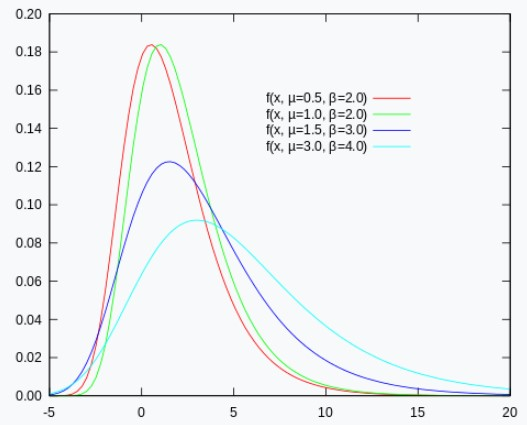
\includegraphics[width=\linewidth]{Probability density function}
\caption*{Probability density function}
\end{minipage}
\hspace{\fill}
\begin{minipage}[h]{0.45\textwidth}
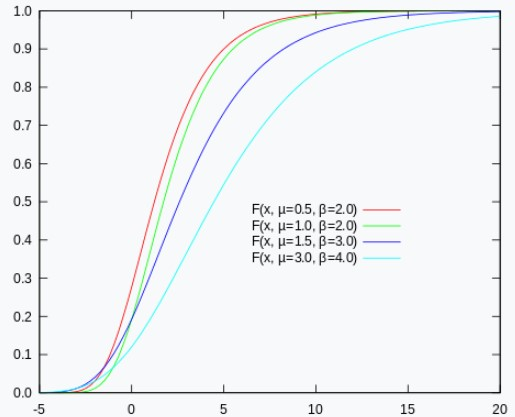
\includegraphics[width=\linewidth]{Cumulative distribution function}
\caption*{Cumulative distribution function}
\label{fig:Gumbel distributionh}
\end{minipage}
\caption{Gumbel distribution} 
\end{figure}

\subsection{Gumbel Softmax Distribution}
Let $Z$ be a categorical variable with categorical distribution Categorical $(\pi_1, …, \pi_x)$, where $\pi_i$ are the class probabilities to be learned by our neural network. Assume our discrete data are encoded as one-hot vectors. The most common way of sampling $Z$ is given by

\begin{equation}
Z = onehot(max\{i | \pi_1 + ... + \pi_{i-1} \leq U\})
\end{equation}

We use softmax as a differentiable approximation to argmax. The sample vectors y are now given by

\begin{equation}
y_i = \frac{exp(\frac{((G_i + log(\pi_i))}{\tau})}{\Sigma_j exp\frac{((G_j + log(\pi_j))}{\tau}}
\label{Gumbel Softmax Distribution}
\end{equation}
where $G_i$ for i = 1,2,...,x are sampled from a Gumbel (0,1) distribution.As $\tau \rightarrow 0$, the softmax computation smoothly approaches the argmax, and the sample vectors approach one-hot; as $\tau \rightarrow \infty$, the sample vectors become uniform. The distribution with the above sampling formula is called the Gumbel-Softmax distribution. Note that continuous vectors are used during training, but the sample vectors are discretized to one-hot vectors during evaluation.



\subsection{Softplus activation function}
It can be viewed as a smooth version of ReLU. The function for Softplus activation function is 
\begin{equation}
f(x) = log(1+exp(x))
\label{Softplus activation function}
\end{equation}

The derivative of softplus is 
\begin{equation}
f'(x) = \frac{1}{1+exp(-x)}
\label{Derivative of Softplus activation function}
\end{equation}

Derivative of Softplus activation function is also called the logistic function.

\begin{figure}[H]
\centering
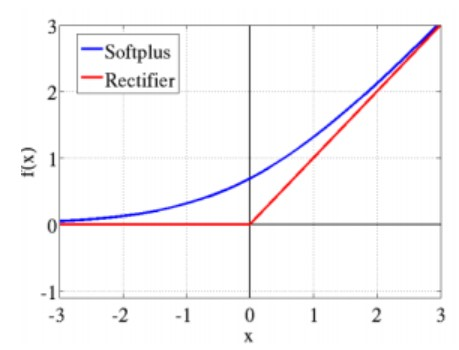
\includegraphics[scale=0.85]{softplus}
\caption{softplus activation function}
\label{fig: softplus}
\end{figure}


\section{VASC: the method overview}

VASC, a generative model based on the Deep Variational Autoencoder (VAE), was developed to find effective low-dimensional representations and facilitate visualization of scRNA-seq datasets. It models the distribution of the high-dimensional original data P(X) via a set of latent variables z. The main purpose of VASC is to find the best z that captures the unique information of the input data. From a probabilistic point of view, given the observed data X, the posterior distribution $P(z|X)$ can be treated as the best distribution of z. However, $P(z|X)$ is usually intractable. Variational inference is thus proposed to solve this problem by designing another common distribution family $Q(z|X)$ (also known as variational distribution) to approximate $P(z|X)$. The minimization of the Kullback–Leibler (KL) divergence between the two distributions is usually adopted for the approximation. The variation distribution $Q(z|X)$ should be sufficiently representative to model the complex information of $P(z|X)$ in the scRNA-seq dataset, while being computationally efficient must be tractable. In VASC, we used a deep neural network to explicitly model the variational distribution. In contrast to traditional methods of variational inference, deep neural networks approximate arbitrary functions and can be efficiently optimized using stochastic gradient descent.

VASC has three major parts, namely, the encoder network, the decoder network, and the zero-inflated (ZI) layer. The encoder network, designed as a three-layer neural network, generates the parameters of the variational distribution. We added a "dropout" noise layer Before the first layers. From a computational point of view, an additional random sound was introduced for sample training for reducing the risk of overfitting during the learning process. 
Assuming a multidimensional Gaussian distribution of $Q(z|X)$ in the latent variable $z$, the mean and variance parameters can be generated by the encoder network from the values $X$ of the given expressions. Then, the learned $Q(z|X)$ was used to re-generate pseudo samples $X'$ by the decoder network, another three-layer neural network.Finally, a ZI layer, based on a double-exponential distribution, was designed to mimic the dropout events by randomly setting some data points as zero.The Gumbel distribution was used in the ZI layer for the back-propagation. VASC was optimized by a stochastic gradient descent-based RMSprop methods to minimize an auxiliary loss function of the KL divergence between $Q(z|X)$ and $P(z|X$). A 2D representation was learned for visualization and other downstream analysis finally.



\section{Overview of VASC:}
\begin{figure}[H]
\centering
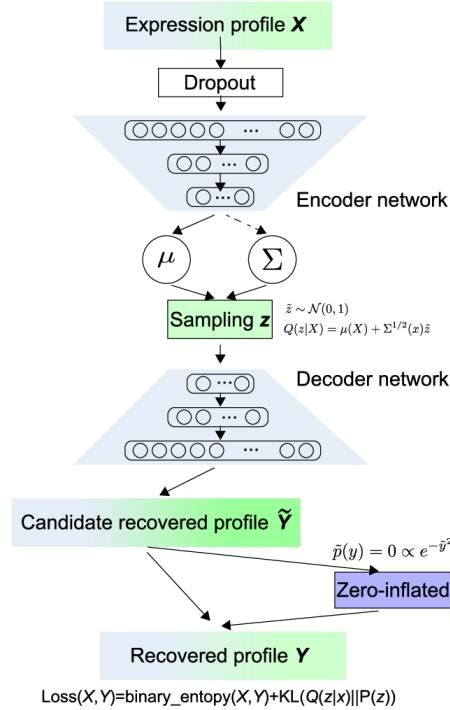
\includegraphics[scale=0.9]{Figure1}
\caption{Overview of VASC workflow(Source : Internet)}
\label{fig: Overview of VASC workflow}
\end{figure}
\clearpage


\section{VAE}
VASC is a deep VAE-based generative model and is designed for the visualization and low-dimensional representation of the scRNA-seq data. VAE aims to model the distribution $P(X)$ of data points in a high-dimensional space $\chi$, with the aid of by minimizing the KL divergence(D) between $Q(z|X)$ and $P(z|X)$ :

\begin{equation}
D[Q(z|X)||P(z|X)] = E_{z\sim Q}[log Q(z|X)- log P(z|X)]
\label{KL Divergent1}
\end{equation}

By applying the Bayes rule and rearranging the order, it can be re-written as

\begin{equation}
log P(X)- D[Q(z|X)||P(z|X)] = E_{z\sim Q}[log P(X|z) - D[Q(z|X)||P(z)]
\label{KL Divergent2}
\end{equation}

where P(X) is a constant and $E_{z\sim Q}$ represents expectation over z that is sampled from Q. Therefore, minimizing the KL divergence is equivalent to maximizing the right-hand part of Equation \ref{KL Divergent2}. The right-hand part has a natural autoencoder structure, with the encoder $Q(z|X)$ from $X$ to $z$ and the decoder $P(X|z)$ from $z$ to $X$. Two deep fully-connected neural networks can be used to model these two parts.

\section{VASC method}
\subsection{Model}
The whole VASC structure is shown in Figure \ref{fig: Overview of VASC workflow}. The model  are described in detail as below.

\subsection*{Input layer}
VASC uses the expression matrix from scRNA-seq data as input. The entire transcriptome expression matrix was directly input into the model without any gene filter applied. The data were log-transformed to make the results more robust. However, the most important transformation was to rescale the expression of each gene in any single cell within the [0,1] range by dividing the maximal expression value of the single gene from the same cell.

\subsection*{Dropout layer}
A dropout layer is added right after the input layer and set the dropout ratio to 0.5. This is larger than the usual choice for deep models in the input layer to improve model training performance. This layer is suitable for scRNA-seq data because it can be viewed as an artificial additional 'dropout' event, forcing subsequent layers to avoid dropout noise.

\subsection*{Encoder network}
The encoder network was designed as a 3-layer fully connected neural network with decreasing dimensions of 512, 128, and 32. The first layer did not use nonlinear activations acting as embedded PCA transforms. Many complex algorithms, including t-SNE, benefit from PCA transforms. An L1 norm regularization was added to the weights in this layer to reduce the sparsity of the model. His next two layers involved ReLU activations, making the output sparse and stable for deep models.


\begin{figure}[H]
\centering
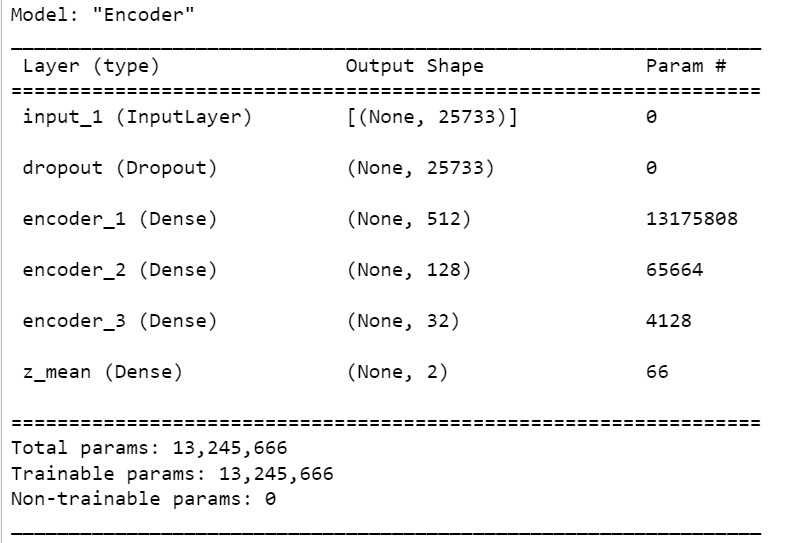
\includegraphics[scale=0.85]{encoder}
\caption{Detail of encoder}
\label{fig: encoder}
\end{figure}


\subsection*{Latent sampling layer}
Latent variables z were modeled by a Gaussian distribution, with the standard normal prior $N(0,I)$. The encoder network was used to estimate its posterior parameters. Usually, both the parameters $\mu$ and $\Sigma$ needed to be estimated, with a linear activation used to estimate $\mu$. According to our experiments, it is better to fix $\Sigma$ and set $log\Sigma = I$, if the dataset only has small sample size. For the datasets with large sample size (more than 1000 cells) $\Sigma$ can also be trained by the encoder network. A ‘softplus’ activation was used for the estimation of $log\Sigma$. Since the neural network does not have a stochastic layer and thus could not be tackled by back-propagation algorithm, a reparameterization trick was used to remove the randomness in input data. It is easy to see, drawing a sample z from $N(\mu, \Sigma)$ is equivalent to drawing a sample $\tilde{z}$ from $N(0,I)$ and
then let $z = \mu + \Sigma^\frac{1}{2}\tilde{z}$

\subsection*{Decoder network}
The decoder network used the generated z to recover the original expression matrix, which was designed as a three-layer fullyconnected neural network with dimensions of hidden units 32, 128, and 512, respectively, and an output layer. The first three layers used ‘ReLU’ activations and the final layer with sigmoid to make the output within [0,1]

\begin{figure}[H]
\centering
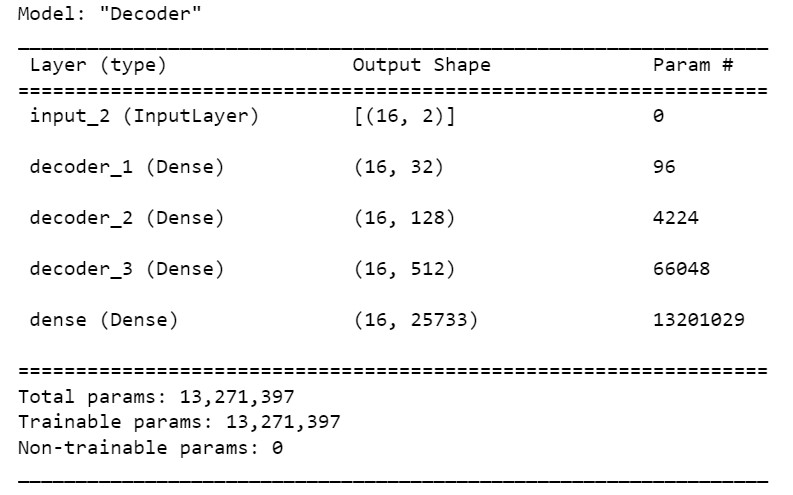
\includegraphics[scale=0.85]{decoder}
\caption{Detail of decoder}
\label{fig: decoder}
\end{figure}

\subsection*{ZI layer}
An additional ZI layer was added after the decoder network. Adapted from the model used by ZIFA, we modeled the dropout events by the probability $e^{-\tilde{y}^2}$ where $\tilde{y}$ is the recovered expression value by the decoder network.Back propagation cannot deal with stochastic units.A Gumbel softmax distribution was introduced to overcome these difficulties.Suppose p is the probability for dropout and $q = 1-p$, the sample s from Gumbel-softmax distribution was obtained by:
\begin{equation}
s = \frac{exp(\frac{((g_0 + log(p))}{\tau})}{exp(\frac{((g_0 + log(p))}{\tau})+exp(\frac{((g_1 + log(q))}{\tau})}
\label{Gumbel-softmax distribution VASC}
\end{equation}
As the hyper-parameter $\tau \rightarrow 0$, the generated samples from the Gumbel-softmax distribution should be identical to the samples from the Bernoulli distribution. In practice, too small values of $\tau$ makes the gradient of the whole network too small and the optimization algorithm cannot work.

\subsection{Loss function}
The loss function as shown in the Equation \ref{KL Divergent2} is composed of
two components. The first part, because of the scale of our data, [0,1], was computed by binary cross-entropy loss function. The second part, controlling the divergence between posterior distribution and the prior $N(0,I)$, could be computed analytically.

\subsection{Optimization}
The whole structure could be optimized end-to-end using the stochastic gradient descent-based optimization algorithm. We chose the RMSprop method for VASC. We set the learning rate as 0.0001. The training processes were stopped if the training loss did not show obvious decrease within 50 epochs.

\subsection{Performance assessment}
To measure the quality of visualization and low-dimensional representation, k-means clustering was applied to the 2D representations of all the aforementioned methods. Then the obtained clustering results were compared with the known cell types provided in the original references. The number of clusters, k, was set to number of known cell types. Four measures were used to assess the performances, including normalized mutual information (NMI), adjusted rand index (ARI), homogeneity, and completeness.

\subsection*{NMI}
Suppose P is the predicted clustering results, and T is the known cell types (the same below), we denote the entropy of P and T as H(P) and H(T), respectively, and the mutual information between them as MI(P,T). NMI is computed as:

\begin{equation}
NMI(P,T) = \frac{MI(P,T}{\sqrt[2]{H(P)H(T)}}
\label{NMI}
\end{equation}

\subsection*{ARI}
Suppose n is the total number of samples, $a_i$ is the number of samples appearing in the i-th cluster of P, $b_j$ is the number of samples appearing in the j-th types of T, and $n_{ij}$ is the number of overlaps between the i-th cluster of P and the j-th type and T. ARI is computed as:

\begin{equation}
ARI = \frac{\Sigma_{ij}{n_{ij} \choose 2}-\frac{\Sigma_i {a_i \choose 2}\Sigma_j {b_j \choose 2}}{{n \choose 2}}}{\frac{1}{2}[\Sigma_i {a_i \choose 2}+ \Sigma_j {b_j \choose 2}]-\frac{\Sigma_i {a_i \choose 2}\Sigma_j {b_j \choose 2}}{{n \choose 2}}}
\label{ARI}
\end{equation}

\subsection*{Homogeneity}
The measure homogeneity expects that every cluster only contains samples from one cell type. Suppose H(T|P) is the crossentropy of cell types given the cluster P, the homogeneity score (h) is computed by:

\begin{equation}
h = 1 - \frac{H(T|P)}{H(T)}
\label{Homogeneity}
\end{equation}

\subsection*{Completeness}
The measure completeness (c) expects that samples from one cell type are assigned to the same cluster, and is computed as:

\begin{equation}
c = 1 - \frac{H(P|T)}{H(P)}
\label{Completeness}
\end{equation}

For all the measures including NMI, ARI, homogeneity, and completeness, larger values (up to 1) mean better performances.

\section{Work on PBMC3k dataset}
\subsection{Analysis of the PBMC3k dataset}
The cells were with less than three detected genes (UMIs > 3). Number of UMI counts was transformed to transcript-per-million (TPM)-like values by normalizing each cell through dividing total UMI counts and then multiplying by 10,000. Log2 transformation was applied after adding a pseudo-count 1 to obtain the gene expression matrix. Due to the serious dropout events present in this dataset, gene selection is used to reduce noises. The same procedure was adopted as previously reported, with 1158 genes that remained. VASC was then tested on this pre-processed gene expression matrix. 

\subsection{Visualization and performance comparison}
The visualization performance of VASC was tested ogether with four state-of-the-art dimension reduction methods, including PCA, t-SNE, ZIFA, and SIMLR.Datasets reported by Goolam et al., Biase et al., and Yan et al., respectively, were generated from studies on the embryonic development from zygote to blast cells. PCA, ZIFA, and VASC roughly re-established the developmental stages of different cell types (cells are expected to be arranged in the order of zygote, 2-cell, 4-cell, 8 cell, 16-cell, and blast cells). However, t-SNE and SIMLR, both of which use neighbor-preserving embedding, showed poor performance on these datasets. In contrast, VASC further separated 16-cell and blast from 8-cell stages in the Goolam dataset. Moreover, compared to PCA and ZIFA, VASC better separated blast cells from 4-cell stages, and identified one zygote as a possible outlier in the Biase dataset, whereas 4-cell stage was better separated from zygote and 2-cell stages using VASC in the Yan dataset. These results indicate that VASC can better model the embryo developmental progression than PCA and ZIFA.

To quantitatively assessing the performance of these methods in dimension reduction and visualization, we compared the cell sub-populations in the reduced subspaces (the sub-populations were identified by k-means clustering) with the true cell type labels annotated in the original publications. Four different parameters were used, including normalized NMI, ARI, homogeneity, and completeness to quantitatively assess the clustering performances. PCA, t-SNE, ZIFA, SIMLR, and VASC were used to systematically analyze the datasets. These comparisons showed that VASC outperformed the other methods in terms of NMI and ARI in most cases. Furthermore, VASC always ranked in the top two methods on all the tested datasets (Figure 3B) in terms of NMI and ARI, respectively. This suggests that VASC has broad compatibility with various kinds of scRNA-seq datasets.

\begin{figure}[H]
\centering
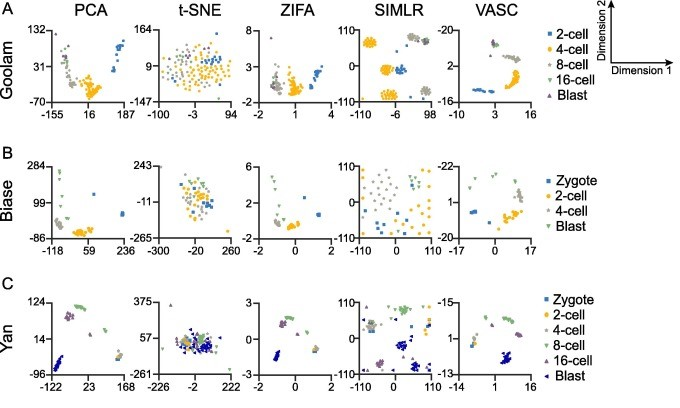
\includegraphics[scale=0.9]{Compare}
\caption{Comparison of various method}
\label{fig: Compare}
\end{figure}

\section{Work on Nestorova16 dataset}
\subsection{Analysis of Nestorova16 dataset}
The dataset is collected from kaggle. It has 1645 data and every data is of 3991 dimensional. There are 3 type of data called 'HSPC','LT.H' and 'Prog'. We fit VASC, tSNE and PCA in this dataset.

\subsection{Visualization}
We fit VASC, t-SNE and PCS on the dataset and we get the graph as follow:

\begin{figure}[H]
\begin{minipage}[h]{0.3\textwidth}
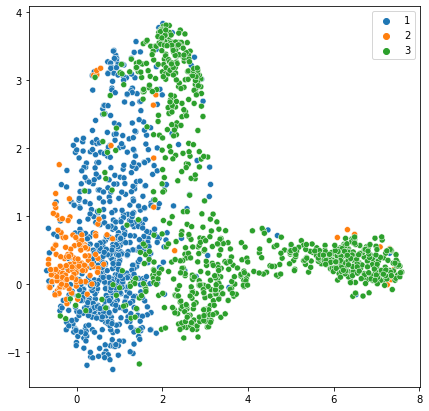
\includegraphics[width=\linewidth]{vasc_graph}
\caption*{VASC}
\end{minipage}
\hspace{\fill}
\begin{minipage}[h]{0.3\textwidth}
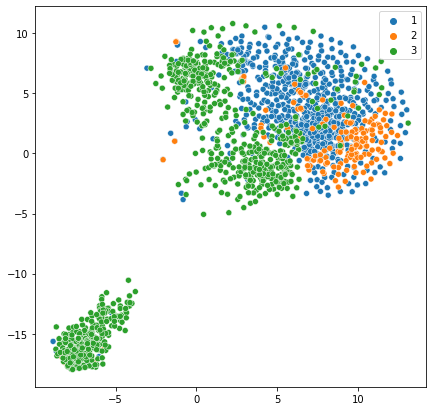
\includegraphics[width=\linewidth]{tSNE}
\caption*{t-SNE}
\label{fig:t-SNE}
\end{minipage}
\begin{minipage}[h]{0.3\textwidth}
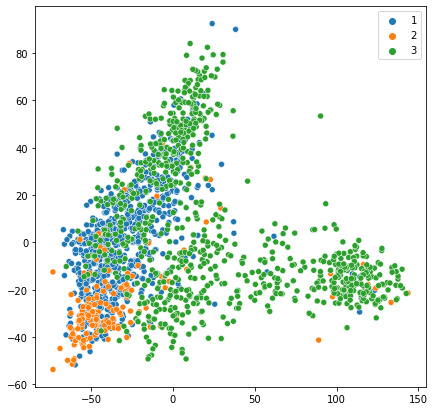
\includegraphics[width=\linewidth]{PCA}
\caption*{PCA}
\end{minipage}
\caption{Visualization of Nestorova16 dataset(Here 1:'HSPC', 2:'LT.H', 3:'Prog')} 
\end{figure}





\section{Conclusion}
In this study, a dimension reduction method, VASC, was developed for scRNA-seq data visualization and analysis.VASC achieves superior performance in most cases and is broadly suitable for different datasets with different data structures in the original space. VASC could make clearer separation of rare cell types than other methods according to data analysis. 

\section{Acknowledgement}
It is needless to say that without the support, encouragement, and friendly care of a number of people this project would not have been possible. We are obligated to ISI,Kolkata for getting us chance and and engaged to this project. We thank all the professors and other stuff of ISI, Kolkata for helping us in every aspects. We want to specially thank to Prof. Rajat K De for his support in understanding the subject and for choosing this paper. We are also thankful to our friends for their unconditional support, inspiration and cooperation. They made our studies more enjoyable, and who could always be consulted with whenever in doubt. It has been a pleasure
to be with them. Wishing them good luck with their future endeavour. Our deepest gratitude is to our parents for their love, affection, encouragement and unfailing emotional support.

\clearpage
\section{References}
\begin{itemize}

\item \href{https://www.sciencedirect.com/science/article/pii/S167202291830439X}{VASC: Dimension Reduction and Visualization of Single-cell RNA-seq Data by Deep Variational Autoencoder by Dongfang Wang, Jin Gu}

\item \href{https://www.frontiersin.org/articles/10.3389/fgene.2019.00317/full}{Single-Cell RNA-Seq Technologies and Related Computational Data Analysis}

\item \href{https://genomemedicine.biomedcentral.com/articles/10.1186/s13073-017-0467-4}{A practical guide to single-cell RNA-sequencing for biomedical research and clinical applications}

\item \href{nature.com/articles/s12276-018-0071-8}{Single-cell RNA sequencing technologies and bioinformatics pipelines}

\item \href{https://en.wikipedia.org/wiki/Gumbel_distribution}{Gumbel distribution}

\item \href{https://towardsdatascience.com/what-is-gumbel-softmax-7f6d9cdcb90e}{What is Gumbel-Softmax}

\item \href{https://neptune.ai/blog/gumbel-softmax-loss-function-guide-how-to-implement-it-in-pytorch}{Gumbel Softmax Loss Function Guide}

\item \href{https://paperswithcode.com/method/softplus}{Softplus}

\item \href{https://sefiks.com/2017/08/11/softplus-as-a-neural-networks-activation-function/}{Softplus as a Neural Networks Activation Function}

\item \href{https://genomebiology.biomedcentral.com/articles/10.1186/s13059-015-0805-z}{ZIFA: Dimensionality reduction for zero-inflated single-cell gene expression analysis}

\item \href{https://bioconductor.org/packages/devel/bioc/vignettes/SIMLR/inst/doc/vignette.pdf}{Single-cell Interpretation via Multi-kernel LeaRning (SIMLR)}

\item \href{https://www.scopus.com/record/display.uri?eid=2-s2.0-1942450753&origin=inward}{Cluster ensembles - A knowledge reuse framework for combining multiple partitions}

\item \href{https://www.scopus.com/record/display.uri?eid=2-s2.0-78649420560&origin=inward}{Information theoretic measures for clusterings comparison: Variants, properties, normalization and correction for chance}

\item \href{https://link.springer.com/article/10.1007/BF01908075}{Comparing partitions}



\end{itemize}


\end{document}
